\documentclass{ximera}
\title{Hints}
\begin{document}

	\begin{abstract}
		Hints can contain questions
	\end{abstract}

\section{Basic hints}
We can add hints to a question to assist students who are having problems

\begin{verbatim}
\begin{question}
  \begin{solution}
    \begin{hint}
      $3 \times 2$ is the number of objects in $3$ groups of $2$ objects
    \end{hint}
    \begin{hint}
      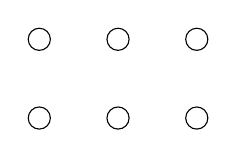
\begin{tikzpicture}
        \draw (0,0) circle (4pt);
        \draw (1,0) circle (4pt);
        \draw (2,0) circle (4pt);
        \draw (0,1) circle (4pt);
        \draw (1,1) circle (4pt);
        \draw (2,1) circle (4pt);
      \end{tikzpicture}
    \end{hint}
    \begin{hint}
      $3\times 2=6$
    \end{hint}
    $3\times 2 = $ \answer{6}
  \end{solution}
\end{question}
\end{verbatim}

\begin{question}
  \begin{solution}
    \begin{hint}
      $3 \times 2$ is the number of objects in $3$ groups of $2$ objects
    \end{hint}
    \begin{hint}
      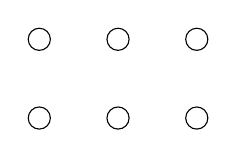
\begin{tikzpicture}
        \draw (0,0) circle (4pt);
        \draw (1,0) circle (4pt);
        \draw (2,0) circle (4pt);
        \draw (0,1) circle (4pt);
        \draw (1,1) circle (4pt);
        \draw (2,1) circle (4pt);
      \end{tikzpicture}
    \end{hint}
    \begin{hint}
      $3\times 2=6$
    \end{hint}
    $3\times 2 = $ \answer{6}
  \end{solution}
\end{question}

\section{Hints with questions}

Hints can also contain further questions! 

\begin{verbatim}
\begin{question}
What is the abscissa of the critical point of the function $f(x) = x^2+2x+1$?
\begin{hint}
\begin{question}
	What is the derivative of $f$?
	\begin{solution}
		$f'(x) = $ \answer{2x+2}
	\end{solution}
\end{question}
\end{hint}
\begin{solution}
	$x = $ \answer{-1}
\end{solution}
\end{question}
\end{verbatim}

\begin{question}
What is the abscissa of the critical point of the function $f(x) = x^2+2x+1$?
\begin{hint}
\begin{question}
	What is the derivative of $f$?
	\begin{solution}
		$f'(x) = $ \answer{2x+2}
	\end{solution}
\end{question}
\end{hint}
\begin{solution}
	$x = $ \answer{-1}
\end{solution}
\end{question}

\end{document}